\documentclass[a4paper,11pt,oneside,titlepage,openany,onecolumn]{scrreprt}

%%%%%%%%%%%%%%%%%%%%%%%%%%%%%%%%%%%%%%%%%%%%%%%%%%%%%%%%%%%%%%%%%%%%%%%%%%%%%%%%%%%%%%

\usepackage{ifthen}
\newboolean{english}
\setboolean{english}{true}


\def\title{Development of a vibrotactile stimulation system for cognitive rehabilitation}
\def\study{Mechatronics \& Smart Technologies}
\def\thesis{Master Thesis}
\def\degree{"Master of Science in Engineering"}
\def\student{Lukas Sieß}
\def\matnr{52010293}
\def\address{6591 Grins, Grins 107H}
\def\reviewerone{Prof. Yeongmi Kim, PhD}


% deutsche Anpassungen
%\usepackage[ansinew]{inputenc}
\usepackage[T1]{fontenc}
\usepackage[ngerman,english]{babel}

% mathematische Symbole
\usepackage{amsmath,amssymb,amsfonts,amstext}

% Listings
\usepackage{listings}
\lstset{numbers=left,numberstyle=\tiny,stepnumber=5,numbersep=5pt}

% erweiterte Zeichenbefehle
\usepackage{pst-all}
\usepackage{hyperref}
\usepackage{glossaries}
\usepackage{booktabs}

% Kopfzeilen frei gestaltbar
\usepackage{fancyhdr}
\lfoot[\fancyplain{}{}]{\fancyplain{}{}}
\rfoot[\fancyplain{}{}]{\fancyplain{}{}}
\cfoot[\fancyplain{}{\footnotesize\thepage}]{\fancyplain{}{\footnotesize\thepage}}
\lhead[\fancyplain{}{\footnotesize\nouppercase\leftmark}]{\fancyplain{}{}}
\chead{}
\rhead[\fancyplain{}{}]{\fancyplain{}{\footnotesize\nouppercase\sc\leftmark}} 

% Farben im Dokument m"oglich
\usepackage{color}

% Schriftart Helvetica
\usepackage{helvet}
\renewcommand{\familydefault}{phv}

% anderdhalbfacher Zeilenabstand
\usepackage{setspace}
\onehalfspacing

% Graphiken einbinden: hier f"ur pdflatex
\usepackage[dvips]{graphicx}

% verbesserte Floating Plazierung
\usepackage{float}

% "Uberpr"ufung des Layouts
\usepackage{layout}

\usepackage{array}

% erweiterte Einstellungen der Bildunterschriften -> 8 Pt
\usepackage[small]{caption}
\captionsetup{belowskip=12pt,aboveskip=4pt}

\usepackage{ifthen}

% H"ohe und Breite des Textk"orpers etwas gr"osser definieren
\usepackage[tmargin=1in,bmargin=1in,lmargin=1.25in,rmargin=1.25in]{geometry}

% Einr"uckung von und Abstand zwischen Abs"atzen
\setlength{\parindent}{0em}
\setlength{\parskip}{1.5ex plus0.5ex minus0.5ex}

% weniger Warnungen wegen "uberf"ullter Boxen
\tolerance = 9999
\sloppy

% Anpassung einiger "Uberschriften 
\renewcommand\figurename{Abbildung}
\renewcommand\tablename{Tabelle}
%\newcommand{\unit}{\mathrm}

% Counter f"ur die Nummerierung
\newcounter{romancount}

% Boolsche Variable f"ur Bachelor-/Masterarbeit oder Bericht
\newboolean{thesis}


\begin{document}

\ifthenelse{\boolean{english}}{\selectlanguage{english}}{\selectlanguage{english}}

%\layout

% Kopf- und Fusszeilen initiieren
\pagestyle{plain}

\pagenumbering{Roman}
\thispagestyle{empty}
\sffamily

\ThisTileWallPaper{\paperwidth}{\paperheight}{Images/MCIHintergrundKPL.pdf}
%\put(-30,-685){\includegraphics[width=1.15\linewidth]{BG}}

{
	\bfseries

	\vspace*{3.5cm}

	\textcolor{MSBlue}{\sffamily\bfseries\huge\thesis}%

	\vspace*{0.5cm}

	\begin{doublespace} 
		
\textbf{\labtitle{} (\labcode)}

\textbf{\labname}

\textbf{\labdate}	

%Labor \labnum

	%\maketitle
	\vspace*{10cm}

	\textcolor{gray}{\study}

	\def\termname{Semester}
	\textcolor{gray}{\term{ }\termname}

	\def\lecturername{Lector}
	\textcolor{gray}{\lecturername: \lecturer}

	\def\groupname{Group}
	\textcolor{gray}{\groupname: \group}

	\def\authorname{Authors}
	\textcolor{gray}{\authorname: \student}

	\textcolor{gray}{\today}
	\end{doublespace} 
	\newpage
}
\thispagestyle{plain} % format page style for current page
\pdfbookmark[0]{Eidesstattliche Erklärung}{Eidesstattliche Erklärung} % sets a PDF bookmark


\chapter*{Eidesstattliche Erklärung}
\glqq Ich erkläre hiermit an Eides statt, dass ich die vorliegende Arbeit selbstständig angefertigt habe. Die aus fremden Quellen direkt oder indirekt übernommenen Gedanken sind als solche kenntlich gemacht. Die Arbeit wurde bisher weder in gleicher noch in ähnlicher Form einer anderen Prüfungsbehörde vorgelegt und auch noch nicht veröffentlicht.\grqq\\[5\baselineskip]
\vspace{2cm}
\begin{tabularx}{\textwidth}{@{}p{5cm}Xp{5cm}@{}} % @{} eliminates default padding
    \hrulefill & & \hrulefill \\
    Ort, Datum & & Unterschrift
\end{tabularx}
%
\section*{\centering \ifthenelse{\boolean{english}}{Acknowledgement}{Danksagung}}
Text Text Text Text Text Text Text Text Text Text Text Text Text Text Text Text Text Text Text Text Text Text Text Text ...
\newpage

\selectlanguage{ngerman}
\section*{\centering Kurzfassung}
Text Text Text Text Text Text Text Text Text Text Text Text Text Text Text Text Text Text Text Text Text Text Text Text ...

% Bitte 3-5 deutsche Schlagw"orter eingeben, die die Arbeit charakterisieren:
\paragraph*{Schlagw"orter:} Schlagwort 1, Schlagwort 2, Schlagwort 3, Schlagwort 4, Schlagwort 5
\newpage

\selectlanguage{english}
\section*{\centering Abstract}
Text Text Text Text Text Text Text Text Text Text Text Text Text Text Text Text Text Text Text Text Text Text Text Text ...

% Bitte 3-5 englische Keywords eingeben, die die Arbeit charakterisieren:
\paragraph*{Keywords:} Keyword 1, Keyword 2, Keyword 3, Keyword 4, Keyword 5

\newpage


\ifthenelse{\boolean{english}}{\selectlanguage{english}}{\selectlanguage{english}}

\tableofcontents%\thispagestyle{empty}
\newpage

\setcounter{romancount}{\value{page}}
\setcounter{page}{1}
\pagenumbering{arabic}

% Kopf- und Fusszeilen initiieren
\pagestyle{fancy}

\selectlanguage{english}

\chapter[Introduction]{Introduction}

\section{Motivation and Problem Statement}

%globale Demenzstatistiken (Alzheimer Int., WHO)
\cite{alzint_dementia_statistics}, \cite{who_dementia_factsheet}

%Bedarf an nicht-pharmakologischen Ansätzen
\cite{Zucchella.2018}

%Frühstudien zur 40-Hz-Stimulati (z.B. Gamma-Wellen, Reduktion von Amyloid in Mäusen)
\cite{Mably.2018}, \cite{Iaccarino.2016}, \cite{Martorell.2019}

\section{Objectives of the Thesis}

Erl"autern Sie an dieser Stelle \emph{genau} was ihre Aufgabe ist. Gegebenfalls grenzen Sie auch die Teile aus, welche nicht im Umfang der Arbeit liegen. Dies kann Ihnen gegen Ende ihrer Arbeit bei der Argumentation helfen.

\section{Structure of the Thesis}

Geben Sie in diesem Abschnitt eine grobe Vorausschau auf den Aufbau der Arbeit. Die Arbeit k"onnte empirisch motiviert sein und mit der Auswertung eines Experimentes beginnen oder theoreitsch und somit logischerweise mit einem Theoriekapitel beginnen.


Etst
\chapter[Formatierungen]{Formatierungen von "Uberschriften und Text in Latex}

In Latex brauchen Sie sich um Formatierungen im Prinzip nicht k"ummern. Es ist lediglich notwendig, dass Sie Kapitel, Abschnitte, Unterabschnitte und so weiter als solche deklarieren.

Multiple Leerzeichen        werden von Latex einfach gel"oscht. Haben Sie einen Absatz beendet (nach 3 bis 4 S"atzen), dann lassen Sie durch ein zweimaliges ''Enter'' eine Zeile Abstand. Der Absatz wird je nach globaler Einstellung einger"uckt oder abgesetzt.

Wollen Sie im Text etwas hervorheben, dann verwenden Sie \emph{hervorgehoben}. Die Hervorhebung wird von Latex automatisch dem jeweiligen Textstil angepasst. Sie k"onnen aber auch etwas explizit \textbf{fett}, \textit{kursiv} oder \underline{unterstrichen} setzen, wobei dies mit Vorsicht zu genie"sen ist.

\section[Abschnitt]{Das wäre ein Abschnitt}

Mit etwas Text ...

\subsection[Unterabschnitt]{Bzw. ein Unterabschnitt}

Wie Ihnen vielleicht schon aufgefallen ist, vergr"o"sert \LaTeX nach einem ''.'' den Abstand geb"uhrlich f"ur ein Satzende. Falls dies nicht ben"otigt wird z.B.~hier, sollte dies h"andisch verhindert werden.

\paragraph{Gliederungsebene 3} Die n"achste Gliederungsebene wird nicht mehr nummeriert.

\LaTeX kennt auch Aufz"ahlungen wobei es diese mit
\begin{enumerate}
\item Nummerierung
\item\label{enum-ebene} auf der ersten Ebene
\item oder
\begin{itemize}
\item ohne Nummerierung
\item auf der 2.~Ebene gibt.
\end{itemize}
\end{enumerate}
Es gibt eine ganze Reihe von weiteren Formatierungsm"oglichkeiten. Z.B.~behandelt {\LaTeX} die erste Seite eines Kapitels anders als alle folgenden. Dies f"allt insbesondere bei der Seitenzahl und der Kopfzeile auf.

\chapter{Analysis of the Current VCA-Based System}

\section{Overview of the Current VCA System}
This section provides an overview of the existing Voice Coil Actuator (VCA)-based setup. The System consists of seven main parts. 

\begin{itemize}
    \item Spring frame (Minimizing the loss of vertical motion transmitted to the node)
    \item Magnet Housing (fixed Magnetic field is always formed)
    \item Bobbin Coil (Magnetic field is formed only when current flows)
    \item Node (Transmitting vertical motion directly to the human body as sound and vibration)
    \item Node screw (fixes the node to the bobbin coil)
    \item Rubber frame (Suppresses vibration from the body from being transmitted to the outside world)
    \item Connection PCB (Take the analog signal from the AMP and apply it to the bobbin coil)
\end{itemize}

\section{Dynamic Behavior: Frequency Measurement}

\subsection{Objective}

\subsection{Measurement Setup}


\subsection{Results \& Interpretation}

\begin{figure}[H]
    \centering
    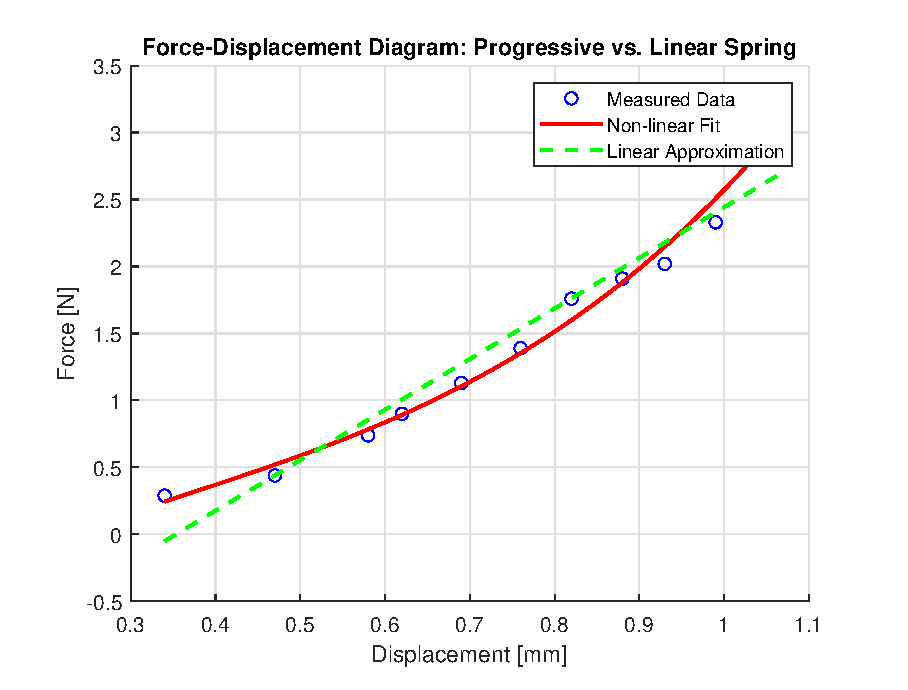
\includegraphics[width=0.62\textwidth]{img/SpringTest.eps}
    \caption[SpringTest]{SpringTest}
    \label{fig:SpringTest}
\end{figure}


\section{Limitations and Identified Challenges}

\chapter[Formatierungen]{Formeln}\label{cha-formeln}

Ein besonderer Vorteil von \LaTeX ist die schnelle und einfache Art Formeln einzugeben. Mit ein wenig "Ubung in der Nomenklatur gehen die komplexesten Ausdr"ucke problemlos von der Hand. Eine einfache Formel sieht folgendermaßen.
\begin{equation}
p_1+\frac{\rho v_1^2}{2}+\rho gh_1=p_2+\frac{\rho v_2^2}{2}+\rho gh_2+\Delta p.
\label{eqn-bernoulli}
\end{equation}
Oft ziehen sich Formeln "uber mehrere Zeilen  
\begin{eqnarray}
\Delta L&=&\int\limits_0^L(1-\cos\varphi)\,dx\approx\int\limits_0^L[1-(1-\varphi^2/2)]\,dx=\frac{1}{2}\int\limits_0^Lw'^2\,dx=\nonumber\\
&=&\frac{B^2\lambda^2}{2}\int\limits_0^L\cos^2\lambda x\,dx=\frac{B^2\lambda^2}{2}\left[\frac{\lambda x-\sin\lambda x\cos\lambda x}{2\lambda}\right]_0^L\approx\frac{B^2\lambda^2L}{4}
\end{eqnarray}
oder sind sehr kompliziert
\begin{eqnarray}
\boldsymbol{\tau}&=&2\mu\mathbf{D}=\mu[\nabla\vec{v}+(\nabla\vec{v})^T]\\
\boldsymbol{\sigma}'&=&\mu'\nabla\cdot\,\vec{v}\,\mathbf{I}=-\frac{2}{3}\mu\,\nabla\cdot(\nabla{v})\,\mathbf{I}.
\end{eqnarray}


\chapter{Evaluation}

\chapter{Zusammenfassung und Ausblick}


\selectlanguage{english}

% This file was created with Citavi 7.0.8.2

@article{Cabral.2024,
 author = {Cabral, Ariana Moura and Lora-Mill{\'a}n, Julio Salvador and Pereira, Adriano Alves and Rocon, Eduardo and Andrade, Adriano de Oliveira},
 abstract = {(1) Background: Vibrotactile stimulation has been studied for tremor, but there is little evidence for Essential Tremor (ET). (2) Methods: This research employed a dataset from a previous study, with data collected from 18 individuals subjected to four vibratory stimuli. To characterise tremor changes before, during, and after stimuli, time and frequency domain features were estimated from the signals. Correlation and regression analyses verified the relationship between features and clinical tremor scores. (3) Results: Individuals responded differently to vibrotactile stimulation. The 250 Hz stimulus was the only one that reduced tremor amplitude after stimulation. Compared to the baseline, the 250 Hz and random frequency stimulation reduced tremor peak power. The clinical scores and amplitude-based features were highly correlated, yielding accurate regression models (mean squared error of 0.09). (4) Conclusions: The stimulation frequency of 250 Hz has the greatest potential to reduce tremors in ET. The accurate regression model and high correlation between estimated features and clinical scales suggest that prediction models can automatically evaluate and control stimulus-induced tremor. A limitation of this research is the relatively reduced sample size.},
 year = {2024},
 title = {{On the Effect of Vibrotactile Stimulation in Essential Tremor}},
 volume = {12},
 number = {4},
 journal = {{Healthcare (Basel, Switzerland)}}
}


@article{Campbell.2022,
 author = {Campbell, Elsa A. and Kantor, Ji{\v{r}}{\'i} and Kantorov{\'a}, Lucia and Svobodov{\'a}, Zuzana and Wosch, Thomas},
 abstract = {The prevalence of dementia is increasing with the ever-growing population of older adults. Non-pharmacological, music-based interventions, including sensory stimulation, were reported by the Lancet Commission in 2020 to be the first-choice approach for managing the behavioural and psychological symptoms of dementia. Low frequency sinusoidal vibration interventions, related to music interventions through their core characteristics, may offer relief for these symptoms. Despite increasing attention on the effectiveness of auditory music interventions and music therapy for managing dementia, this has not included low frequency vibration. This scoping review, following the JBI methodology guidelines, was conducted to investigate participants' responses to both sound and mechanical vibration, the characteristics of the delivered interventions, methodological challenges, and the specifics of the research experiments reported. An extensive search was conducted in BMC, CINAHL, Cochrane Central Register of Controlled Trials, EMBASE, ERIC, MEDLINE (OvidSP), Pedro, ProQuest Central, PsycINFO, Scopus, and Web of Science. Current Controlled Trials, Clinical Trials, and Google Scholar were also searched as well as a hand search in relevant journals. Studies on adults with all types of dementia, investigating tactile low frequency sound or mechanical vibration in any context were considered. Data from eight full-length studies (three RCTs, two quasi-experimental, two case reports, and one qualitative) were extracted using the data extraction table developed by the authors and were included in the analysis and critical appraisal. Issues in quality related to, for example, control groups and blinding. Few studies addressed participants' subjective responses to the interventions. Reporting on the intervention characteristics was unclear. It appeared more frequent sessions led to better outcomes and home-based interventions potentially addressing the issue of access and feasibility. Future research should include neuroimaging to measure and confirm the hypothesised mechanism of cerebral coherence. Standardised reporting of intervention characteristics is also needed to ensure replicability of the experiments. Higher quality research is needed to investigate the impact and effect of low frequency vibration for the symptoms of dementia and compare outcomes in meta-syntheses.},
 year = {2022},
 title = {{Tactile Low Frequency Vibration in Dementia Management: A Scoping Review}},
 pages = {854794},
 volume = {13},
 journal = {{Frontiers in psychology}}
}


@article{Clair.1993,
 author = {Clair, A. A. and Bernstein, B.},
 year = {1993},
 title = {{The Preference for Vibrotactile Versus Auditory Stimuli in Severely Regressed Persons with Dementia of the Alzheimer's Type Compared to Those with Dementia due to Alcohol Abuse}},
 pages = {24--27},
 volume = {11},
 number = {1},
 journal = {{Music Therapy Perspectives}}
}


@article{ClementsCortes.2016,
 author = {Clements-Cortes, Amy and Ahonen, Heidi and Evans, Michael and Freedman, Morris and Bartel, Lee},
 abstract = {This study assessed the effect of stimulating the somatosensory system of Alzheimer's disease (AD) patients at three stages of their illness with 40 Hz sound. In this AB cross-over study design, 18 participants (6 mild, 6 moderate, 6 severe) each participated in 13 sessions: one intake and 12 treatment. Treatment A consisted of 40 Hz sound stimulation and Treatment B consisted of visual stimulation using DVDs, each provided twice a week over 6 weeks for a total of 6 times per treatment. Outcome measures included: St. Louis University Mental Status Test (SLUMS), Observed Emotion Rating Scale, and behavioral observation by the researcher. Data were submitted to regression analysis for the series of 6 SLUMS scores in treatment A and 6 scores in B with comparison by group. The slopes for the full sample and subgroups in the 40 Hz treatment were all significant beyond alpha = 0.05, while those for the DVD were not. A thematic analysis of qualitative observations supported the statistical findings. 40 Hz treatment appeared to have the strongest impact on persons with mild and moderate AD. Results are promising in terms of a potential new treatment for persons with AD, and further research is needed.},
 year = {2016},
 title = {{Short-Term Effects of Rhythmic Sensory Stimulation in Alzheimer's Disease: An Exploratory Pilot Study}},
 pages = {651--660},
 volume = {52},
 number = {2},
 journal = {{Journal of Alzheimer's disease : JAD}}
}


@article{ClementsCortes.2017,
 author = {Clements-Cortes, Amy and Bartel, Lee and Ahonen, Heidi and Freedman, Morris and Evans, Michael and Tang-Wai, David},
 year = {2017},
 title = {{Can Rhythmic Sensory Stimulation Decrease Cognitive Decline in Alzheimer's Disease?: A Clinical Case Study}},
 pages = {174},
 volume = {9},
 number = {3},
 journal = {{Music and Medicine}}
}


@article{ClementsCortes.2017b,
 author = {Clements-Cortes, Amy and Bartel, Lee and Ahonen, Heidi and Freedman, Morris},
 year = {2017},
 title = {{The Potential of Rhythmic Sensory Stimulation Treatments for Persons with Alzheimer's Disease}},
 pages = {167},
 volume = {9},
 number = {3},
 journal = {{Music and Medicine}}
}


@article{ClementsCortes.2022,
 author = {Clements-Cortes, Amy and Bartel, Lee},
 abstract = {Dementia prevalence is increasing globally, and symptom management and treatment strategies require further investigation. Music-based interventions have demonstrated some efficacy with respect to quality of life and symptom reduction, though limited with respect to cognition. This study reports on three case studies where the use of gamma stimulation over one year contributed to maintenance of cognition and increases in mood for participants with Alzheimer's disease or mild cognitive impairment. Auditory stimulation with isochronous sound at 40 Hz was delivered to participants via a commercially available vibroacoustic chair device five times per week for 30 min with assistance from caregivers. Further research is needed to assess the integration of this therapy in the overall care for persons with dementia.},
 year = {2022},
 title = {{Long-Term Multi-Sensory Gamma Stimulation of Dementia Patients: A Case Series Report}},
 volume = {19},
 number = {23},
 journal = {{International journal of environmental research and public health}}
}


@article{Guger.2012,
 author = {Guger, Christoph and Krausz, Gunther and Allison, Brendan Z. and Edlinger, Guenter},
 abstract = {Most brain-computer interfaces (BCIs) rely on one of three types of signals in the electroencephalogram (EEG): P300s, steady-state visually evoked potentials, and event-related desynchronization. EEG is typically recorded non-invasively with electrodes mounted on the human scalp using conductive electrode gel for optimal impedance and data quality. The use of electrode gel entails serious problems that are especially pronounced in real-world settings when experts are not available. Some recent work has introduced dry electrode systems that do not require gel, but often introduce new problems such as comfort and signal quality. The principal goal of this study was to assess a new dry electrode BCI system in a very common task: spelling with a P300 BCI. A total of 23 subjects used a P300 BCI to spell the word {\textquotedbl}LUCAS{\textquotedbl} while receiving real-time, closed-loop feedback. The dry system yielded classification accuracies that were similar to those obtained with gel systems. All subjects completed a questionnaire after data recording, and all subjects stated that the dry system was not uncomfortable. This is the first field validation of a dry electrode P300 BCI system, and paves the way for new research and development with EEG recording systems that are much more practical and convenient in field settings than conventional systems.},
 year = {2012},
 title = {{Comparison of dry and gel based electrodes for p300 brain-computer interfaces}},
 pages = {60},
 volume = {6},
 journal = {{Frontiers in neuroscience}}
}


@article{Guger.2017,
 author = {Guger, Christoph and Spataro, Rossella and Allison, Brendan Z. and Heilinger, Alexander and Ortner, Rupert and Cho, Woosang and {La Bella}, Vincenzo},
 abstract = {Many patients with locked-in syndrome (LIS) or complete locked-in syndrome (CLIS) also need brain-computer interface (BCI) platforms that do not rely on visual stimuli and are easy to use. We investigate command following and communication functions of mindBEAGLE with 9 LIS, 3 CLIS patients and three healthy controls. This tests were done with vibro-tactile stimulation with 2 or 3 stimulators (VT2 and VT3 mode) and with motor imagery (MI) paradigms. In VT2 the stimulators are fixed on the left and right wrist and the participant has the task to count the stimuli on the target hand in order to elicit a P300 response. In VT3 mode an additional stimulator is placed as a distractor on the shoulder and the participant is counting stimuli either on the right or left hand. In motor imagery mode the participant is instructed to imagine left or right hand movement. VT3 and MI also allow the participant to answer yes and no questions. Healthy controls achieved a mean assessment accuracy of 100{\%} in VT2, 93{\%} in VT3, and 73{\%} in MI modes. They were able to communicate with VT3 (86.7{\%}) and MI (83.3{\%}) after 2 training runs. The patients achieved a mean accuracy of 76.6{\%} in VT2, 63.1{\%} in VT3, and 58.2{\%} in MI modes after 1-2 training runs. 9 out of 12 LIS patients could communicate by using the vibro-tactile P300 paradigms (answered on average 8 out of 10 questions correctly) and 3 out of 12 could communicate with the motor imagery paradigm (answered correctly 4,7 out of 5 questions). 2 out of the 3 CLIS patients could use the system to communicate with VT3 (90 and 70{\%} accuracy). The results show that paradigms based on non-visual evoked potentials and motor imagery can be effective for these users. It is also the first study that showed EEG-based BCI communication with CLIS patients and was able to bring 9 out of 12 patients to communicate with higher accuracies than reported before. More importantly this was achieved within less than 15-20 min.},
 year = {2017},
 title = {{Complete Locked-in and Locked-in Patients: Command Following Assessment and Communication with Vibro-Tactile P300 and Motor Imagery Brain-Computer Interface Tools}},
 pages = {251},
 volume = {11},
 journal = {{Frontiers in neuroscience}}
}


@article{Heesterbeek.2019,
 author = {Heesterbeek, Marelle and {van der Zee}, Eddy Anton and {van Heuvelen}, Marieke Joan Gerda},
 abstract = {BACKGROUND

Increasing physical activity levels in patients with dementia can reduce pathology severity and progression of the disease. However, physical activity programs can be challenging to adhere to for this vulnerable population. Three novel forms of passive exercise in a multisensory environment may be feasible alternatives for patients who can no longer be involved in physical activity.

OBJECTIVE

To determine the feasibility of three different forms of passive exercise in a multisensory environment in inactive institutionalized older adults with dementia.

METHODS

120 patients with dementia participated in this single blind randomized controlled trial (64.5{\%} female, age 85.3$\pm$6.8 years Mini-Mental State Examination range 0-29). Ninety participants were randomly assigned to one of the three intervention groups: Therapeutic Motion Simulation (TMSim), Whole Body Vibration (WBV), and TMSim + WBV. Participants received 6 weeks of passive exercise, 4 sessions a week, 4 (WBV) to 12 (TMSim and TMSim + WBV) minutes per session. Feasibility of the novel forms of passive exercise was evaluated based on attendance, compliance, (proxy) experience scores, adverse events and drop-out rates.

RESULTS

On average 87.9{\%} of the offered intervention sessions were attended. All three forms of passive exercise were well appreciated by the participants (7.3 on a scale from 0 to 10). Intervention related drop-out rates were reasonable (12.2{\%}) and no serious adverse events occurred.

CONCLUSION

The novel passive exercise interventions TMSim, WBV, and TMSim + WBV are feasible to apply in patients at all stages of dementia. More research is needed to establish effectiveness of passive exercise to limit adverse effects of dementia.},
 year = {2019},
 title = {{Feasibility of Three Novel Forms of Passive Exercise in a Multisensory Environment in Vulnerable Institutionalized Older Adults with Dementia}},
 pages = {681--690},
 volume = {70},
 number = {3},
 journal = {{Journal of Alzheimer's disease : JAD}}
}


@article{Iaccarino.2016,
 author = {Iaccarino, Hunter F. and Singer, Annabelle C. and Martorell, Anthony J. and Rudenko, Andrii and Gao, Fan and Gillingham, Tyler Z. and Mathys, Hansruedi and Seo, Jinsoo and Kritskiy, Oleg and Abdurrob, Fatema and Adaikkan, Chinnakkaruppan and Canter, Rebecca G. and Rueda, Richard and Brown, Emery N. and Boyden, Edward S. and Tsai, Li-Huei},
 abstract = {Changes in gamma oscillations (20-50 Hz) have been observed in several neurological disorders. However, the relationship between gamma oscillations and cellular pathologies is unclear. Here we show reduced, behaviourally driven gamma oscillations before the onset of plaque formation or cognitive decline in a mouse model of Alzheimer's disease. Optogenetically driving fast-spiking parvalbumin-positive (FS-PV)-interneurons at gamma (40 Hz), but not other frequencies, reduces levels of amyloid-\textgreek{b} (A\textgreek{b})1-40 and A\textgreek{b} 1-42 isoforms. Gene expression profiling revealed induction of genes associated with morphological transformation of microglia, and histological analysis confirmed increased microglia co-localization with A\textgreek{b}. Subsequently, we designed a non-invasive 40 Hz light-flickering regime that reduced A\textgreek{b}1-40 and A\textgreek{b}1-42 levels in the visual cortex of pre-depositing mice and mitigated plaque load in aged, depositing mice. Our findings uncover a previously unappreciated function of gamma rhythms in recruiting both neuronal and glial responses to attenuate Alzheimer's-disease-associated pathology.},
 year = {2016},
 title = {{Gamma frequency entrainment attenuates amyloid load and modifies microglia}},
 pages = {230--235},
 volume = {540},
 number = {7632},
 journal = {{Nature}}
}


@article{Kim.2018,
 author = {Kim, Ki-Hong and Lee, Hyang-Beum},
 abstract = {This study conducted the Korean version of Mini-Mental State Examination (MMSE-K) to women aged 65 or older residing in Gangwon-do Province and screened those who were suspicious to have mild dementia for receiving 23 points or lower in it. For eight weeks, this author tried to verify the effects of whole body vibration exercise intervention on electroencephalogram (EEG) activation and cognitive function in women with senile dementia. According to the results, both EEG activation and cognitive function indicated statistically significant difference in terms of the interactive effect between the measuring times and groups, and there was statistically significant improvement found after the whole body vibration exercise intervention. The results of this study are meaningful because they present the possibility of whole body vibration exercise intervention to be integrated into the plan to improve life quality in patients with senile dementia by stimulating their muscle spindles and sensory organs only with the amplitude and the number of vibrations with no burden of physical activity and enhancing their EEG activation and cognitive function through the responses of the neuromuscular system.},
 year = {2018},
 title = {{The effects of whole body vibration exercise intervention on electroencephalogram activation and cognitive function in women with senile dementia}},
 pages = {586--591},
 volume = {14},
 number = {4},
 journal = {{Journal of exercise rehabilitation}}
}


@article{Lam.2018,
 author = {Lam, Freddy M. H. and Liao, L. R. and Kwok, Timothy C. Y. and Pang, Marco Y. C.},
 abstract = {OBJECTIVE

To evaluate the effects of whole-body vibration (WBV) added to a routine activity program on lower limb strength, balance, and mobility among community-dwelling individuals with mild or moderate dementia, compared with the routine program alone.

METHODS

Fifty-four older adults (40 women; mean (SD) age: 79.8 (6.1) years) with mild or moderate dementia were recruited from two daycare centers. The participants were randomly allocated to undergo a routine day activity program combined with WBV training (WBV at 30 Hz, 2-mm peak-to-peak amplitude) or the routine program only without WBV for 9 weeks (18 sessions). The primary outcome was functional mobility, measured using the timed up-and-go test. The following secondary outcomes were evaluated: Berg Balance Scale, Tinetti balance assessment, time to complete 5 repetitions of sit-to-stand, Quality of Life in Alzheimer's disease questionnaire, and Activities-specific Balance Confidence scale. The attendance rate and incidence of adverse events were also recorded.

RESULTS

The attendance rate for the training was high (86.0{\%}). The incidence of adverse events was low, with only two of the 27 participants in the WBV group reporting mild knee pain. While significant improvement in timed up-and-go, Berg Balance Scale, and Tinetti balance score was found in both groups, none of the outcomes demonstrated a significant group by time interaction.

CONCLUSIONS

WBV training is feasible and safe to use with people with mild or moderate dementia. However, it did not lead to further improvement in physical function and quality of life than the usual activity program provided at the daycare centers. Copyright {\copyright} 2017 John Wiley {\&} Sons, Ltd.},
 year = {2018},
 title = {{Effects of adding whole-body vibration to routine day activity program on physical functioning in elderly with mild or moderate dementia: a randomized controlled trial}},
 pages = {21--30},
 volume = {33},
 number = {1},
 journal = {{International journal of geriatric psychiatry}}
}


@article{Mably.2018,
 author = {Mably, Alexandra J. and Colgin, Laura Lee},
 abstract = {Gamma oscillations ($\sim$25-100 Hz) are believed to play a role in cognition. Accordingly, aberrant gamma oscillations have been observed in several cognitive disorders, including Alzheimer's disease and Fragile X syndrome. Here, we review how recent results showing abnormal gamma rhythms in Alzheimer's disease and Fragile X syndrome help reveal links between cellular disturbances and cognitive impairments. We also discuss how gamma results from rodent models of Alzheimer's disease and Fragile X syndrome may provide insights about unique functions of distinct slow ($\sim$25-50 Hz) and fast gamma ($\sim$55-100 Hz) subtypes. Finally, we consider studies employing brain stimulation paradigms in Alzheimer's disease and discuss how such studies may reveal causal relationships between gamma impairments and memory disturbances.},
 year = {2018},
 title = {{Gamma oscillations in cognitive disorders}},
 pages = {182--187},
 volume = {52},
 journal = {{Current opinion in neurobiology}}
}


@article{Martorell.2019,
 author = {Martorell, Anthony J. and Paulson, Abigail L. and Suk, Ho-Jun and Abdurrob, Fatema and Drummond, Gabrielle T. and Guan, Webster and Young, Jennie Z. and Kim, David Nam-Woo and Kritskiy, Oleg and Barker, Scarlett J. and Mangena, Vamsi and Prince, Stephanie M. and Brown, Emery N. and Chung, Kwanghun and Boyden, Edward S. and Singer, Annabelle C. and Tsai, Li-Huei},
 abstract = {We previously reported that inducing gamma oscillations with a non-invasive light flicker (gamma entrainment using sensory stimulus or GENUS) impacted pathology in the visual cortex of Alzheimer's disease mouse models. Here, we designed auditory tone stimulation that drove gamma frequency neural activity in auditory cortex (AC) and hippocampal CA1. Seven days of auditory GENUS improved spatial and recognition memory and reduced amyloid in AC and hippocampus of 5XFAD mice. Changes in activation responses were evident in microglia, astrocytes, and vasculature. Auditory GENUS also reduced phosphorylated tau in the P301S tauopathy model. Furthermore, combined auditory and visual GENUS, but not either alone, produced microglial-clustering responses, and decreased amyloid in medial prefrontal cortex. Whole brain analysis using SHIELD revealed widespread reduction of amyloid plaques throughout neocortex after multi-sensory GENUS. Thus, GENUS can be achieved through multiple sensory modalities with wide-ranging effects across multiple brain areas to improve cognitive function.},
 year = {2019},
 title = {{Multi-sensory Gamma Stimulation Ameliorates Alzheimer's-Associated Pathology and Improves Cognition}},
 pages = {256-271.e22},
 volume = {177},
 number = {2},
 journal = {{Cell}}
}


@article{Mercado.2006,
 author = {Mercado, C. and Mercado, E.},
 year = {2006},
 title = {{A Program Using Environmental Manipulation, Music Therapy Activities, and the Somatron(C) Vibroacoustic Chair To Reduce Agitation Behaviors of Nursing Home Residents with Psychiatric Disorders}},
 pages = {30--38},
 volume = {24},
 number = {1},
 journal = {{Music Therapy Perspectives}}
}


@article{SebastianRomagosa.2020,
 author = {Sebasti{\'a}n-Romagosa, Marc and Udina, Esther and Ortner, Rupert and Dinar{\`e}s-Ferran, Josep and Cho, Woosang and Murovec, Nensi and Matencio-Peralba, Clara and Sieghartsleitner, Sebastian and Allison, Brendan Z. and Guger, Christoph},
 abstract = {INTRODUCTION

Recent studies explored promising new quantitative methods to analyze electroencephalography (EEG) signals. This paper analyzes the correlation of two EEG parameters, Brain Symmetry Index (BSI) and Laterality Coefficient (LC), with established functional scales for the stroke assessment.

METHODS

Thirty-two healthy subjects and thirty-six stroke patients with upper extremity hemiparesis were recruited for this study. The stroke patients where subdivided in three groups according to the stroke location: Cortical, Subcortical, and Cortical + Subcortical. The participants performed assessment visits to record the EEG in the resting state and perform functional tests using rehabilitation scales. Then, stroke patients performed 25 sessions using a motor-imagery based Brain Computer Interface system (BCI). BSI was calculated with the EEG data in resting state and LC was calculated with the Event-Related Synchronization maps.

RESULTS

The results of this study demonstrated significant differences in the BSI between the healthy group and Subcortical group (P = 0.001), and also between the healthy and Cortical+Subcortical group (P = 0.019). No significant differences were found between the healthy group and the Cortical group (P = 0.505). Furthermore, the BSI analysis in the healthy group based on gender showed statistical differences (P = 0.027). In the stroke group, the correlation between the BSI and the functional state of the upper extremity assessed by Fugl-Meyer Assessment (FMA) was also significant, \textgreek{r} = -0.430 and P = 0.046. The correlation between the BSI and the FMA-Lower extremity was not significant (\textgreek{r} = -0.063, P = 0.852). Similarly, the LC calculated in the alpha band has significative correlation with FMA of upper extremity (\textgreek{r} = -0.623 and P {\textless} 0.001) and FMA of lower extremity (\textgreek{r} = -0.509 and P = 0.026). Other important significant correlations between LC and functional scales were observed. In addition, the patients showed an improvement in the FMA-upper extremity after the BCI therapy (\textgreek{D}FMA = 1 median [IQR: 0-8], P = 0.002).

CONCLUSION

The quantitative EEG tools used here may help support our understanding of stroke and how the brain changes during rehabilitation therapy. These tools can help identify changes in EEG biomarkers and parameters during therapy that might lead to improved therapy methods and functional prognoses.},
 year = {2020},
 title = {{EEG Biomarkers Related With the Functional State of Stroke Patients}},
 pages = {582},
 volume = {14},
 journal = {{Frontiers in neuroscience}}
}


@article{Zucchella.2018,
 author = {Zucchella, Chiara and Sinforiani, Elena and Tamburin, Stefano and Federico, Angela and Mantovani, Elisa and Bernini, Sara and Casale, Roberto and Bartolo, Michelangelo},
 abstract = {Background: Alzheimer's disease (AD) and dementia are chronic diseases with progressive deterioration of cognition, function, and behavior leading to severe disability and death. The prevalence of AD and dementia is constantly increasing because of the progressive aging of the population. These conditions represent a considerable challenge to patients, their family and caregivers, and the health system, because of the considerable need for resources allocation. There is no disease modifying intervention for AD and dementia, and the symptomatic pharmacological treatments has limited efficacy and considerable side effects. Non-pharmacological treatment (NPT), which includes a wide range of approaches and techniques, may play a role in the treatment of AD and dementia. Aim: To review, with a narrative approach, current evidence on main NPTs for AD and dementia. Methods: PubMed and the Cochrane database of systematic reviews were searched for studies written in English and published from 2000 to 2018. The bibliography of the main articles was checked to detect other relevant papers. Results: The role of NPT has been largely explored in AD and dementia. The main NPT types, which were reviewed here, include exercise and motor rehabilitation, cognitive rehabilitation, NPT for behavioral and psychological symptoms of dementia, occupational therapy, psychological therapy, complementary and alternative medicine, and new technologies, including information and communication technologies, assistive technology and domotics, virtual reality, gaming, and telemedicine. We also summarized the role of NPT to address caregivers' burden. Conclusions: Although NPT is often applied in the multidisciplinary approach to AD and dementia, supporting evidence for their use is still preliminary. Some studies showed statistically significant effect of NPT on some outcomes, but their clinical significance is uncertain. Well-designed randomized controlled trials with innovative designs are needed to explore the efficacy of NPT in AD and dementia. Further studies are required to offer robust neurobiological grounds for the effect of NPT, and to examine its cost-efficacy profile in patients with dementia.},
 year = {2018},
 title = {{The Multidisciplinary Approach to Alzheimer's Disease and Dementia. A Narrative Review of Non-Pharmacological Treatment}},
 pages = {1058},
 volume = {9},
 journal = {{Frontiers in neurology}}
}




% Anh"ange
\selectlanguage{english}
\begin{appendix}
	\chapter[Erster Anhang]{Überschrift des ersten Anhangs}\label{app-A}

\lstinputlisting[caption={Test}, label={lst:test_code}]{code/matlab_example.m}


	\chapter[Erster Anhang]{Überschrift des ersten Anhangs}\label{app-A}

\lstinputlisting[caption={Test}, label={lst:test_code}]{code/matlab_example.m}


\end{appendix}

\end{document}
